\subsection{Examples}
\cite{RAUSCH2014556} analyze the distributional impact of implementing clean electricity standards across regions and households. They employ the following utility function
\begin{align}
   U_{rh} = [\mu_{cr}^h \text{min}[g^h(C_{1rh},C_{2rh},...,C_{Irh}),\text{min}(I{1rh},...,I{Irh})]^{1/\rho_cr} + \gamma_{cr}^h N_{rh}^{1/\rho_cr}]^{1/\rho_cr},
\end{align}
where $r$ represents region, $h$ represents income class, $\mu$ and $\gamma$ are CES share coefficients. $g^h(\cdot)$ is a CES composite of different goods, as in \citep{paltsev2005emissions}. The CES nest structure is described in the following figure
\begin{figure}[H]
\centering
\caption{\cite{paltsev2005emissions} CES nest structure}
\label{paltsev nest}
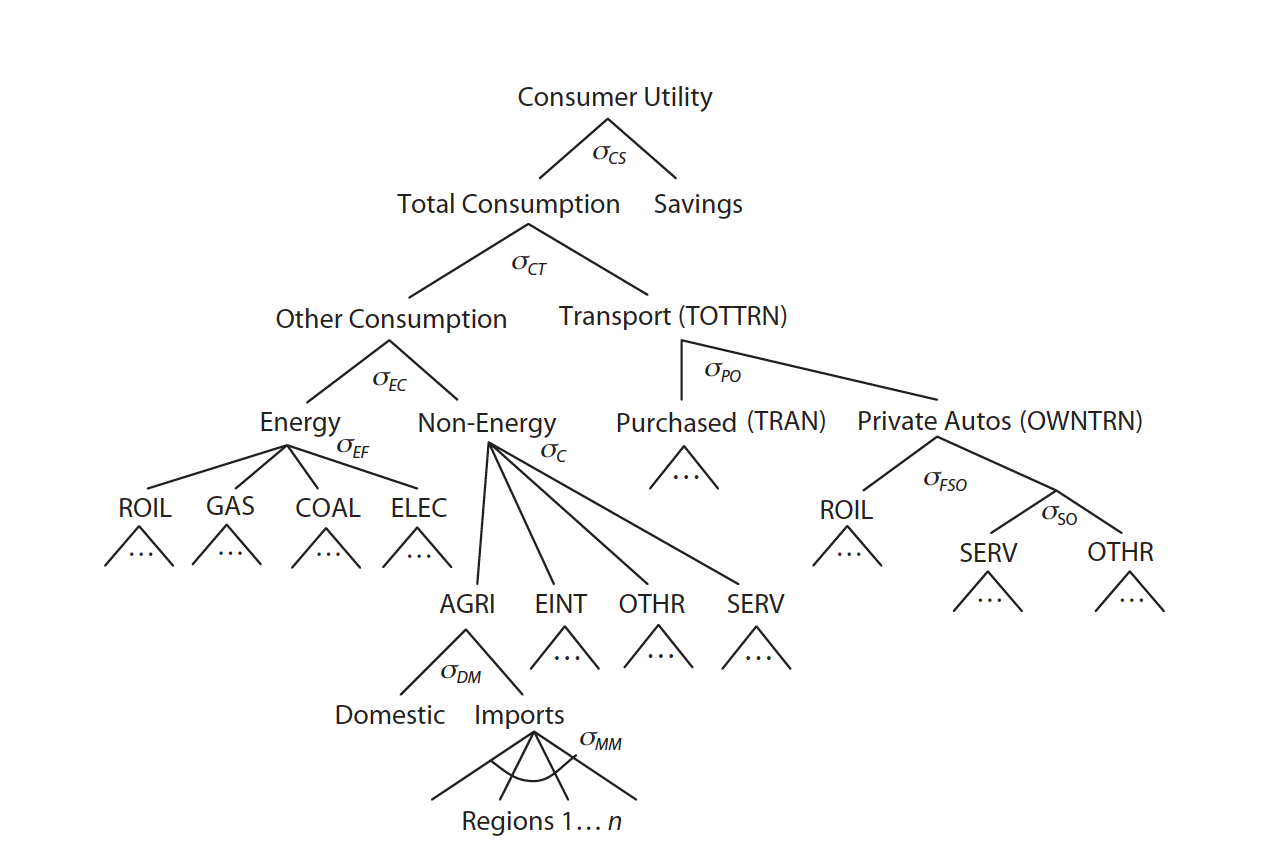
\includegraphics[width=\textwidth]{Screenshots/paltsev CES-nest.png}
\captionsetup{singlelinecheck=off,size=scriptsize}
\setlength{\captionmargin}{10pt}
\caption*{
\textbf{Note:} Nest structure\\
\textbf{Source:} \cite{paltsev2005emissions}}
\end{figure}



\subsection{The CDE Demand System}
Consider an expenditure function C, a price vector p and a Hicksian demand vector q. The expenditure function is chosen to minimize expenditure for given preferences and income (?). The benchmark condition is denoted with the subscript 0: \(c_0=C(p_0,u)={min p_0q_0:f(q_0)\geq u}\), where u is utility. Normalizing the expenditure function with the benchmark condition, it becomes equal to 1: \(C(p_0/c_0)=1\). Hanoch (1975) proposed the expenditure function of a Constant Difference Elasticity demand system as follows (Chen 2017): 
\begin{equation}
    C(\frac{p}{c_0},u)=\sum_i\beta_i u^{e_i (1-\alpha_i)} (\frac{p_i}{c_0})^{1-\alpha_i}=1
\end{equation}
where i denotes each commodity, \(\alpha_i\) is the substitution parameter for good i, \(e_i\) is the expansion parameter for good i. Utility is only indirectly defined. 
The corresponding Hicksian demand for commodity i is given by: 
\begin{equation}
q_i=\frac{\beta_i u^{e_i(1-\alpha_i)}(1-\alpha_i)(\frac{p_i}{c_0})^{-\alpha_i}}{\sum_j\beta_j u^{e_j (1-\alpha_j)}(1-\alpha_j)(\frac{p_j}{c_0})^{(1-\alpha_j)}}
\end{equation}Kan u godt erstattes af indkomst? \(\beta\) is a budget share parameter. When p increases for some commodity i, the effect on q is dependent on substitution parameter for the given commodity. If the substitution parameter is zero, there is no price effect (except for if u is changed?) and if the substitution parameter is large, the price increase will result in a larger drop in q. This effect is further dependent on the utility (income?) and expenditure parameter. If the expansion parameter is high for the given commodity, the higher is the effect of the price increase.

\textit{Det ville være nemt hvis u var disponibel indkomst, alpha substitutionselasticitet og e indkomstelasticitet :)
Skulle man så estimere 30 sub elasticiteter, for hver indkomstgruppe, hvis man har 6 goder?
+ 6 ind elast. 
Kalibrering ser rimelig voldsomt ud, men der er noget kode tilgængeligt.}

\subsection{The LES demand system}
The Linear Expenditure System (LES) is a generalization of a Cobb-Douglas utility form. It contains a treshold \(b\) representing a minimum consumption level for each good. In the %Cobb-Douglas case this treshold is set equal to zero. 
\begin{equation}
U(X)=\prod_{i=1}^n (X_i-b_i)^{\alpha_i}
\end{equation}Consumers allocate income to cover the minimum consumption level and only further consumption enters the function for consumer preferences. The Marshallian demand is given by:
\begin{equation}
X_i = b_i+\frac{\alpha_i}{P_i}(m_h-\sum_i P_j b_j)
\end{equation}where \(m_h\) is the income for household h and the term \((m_h-\sum_iP_j\mu_j)\) denotes the income available %after subsistence consumption. 

\subsection{Experiments in GAMS}
We set up a model in GAMS, with a simple linear production sector, two goods (clean and dirty, $f=C,D$, and two consumers (low- and high income, $hh=L,H$). Each  each allocated an unequal share of income. Consumers optimize a CES utility function with two inputs.

Demand for goods are given as
\begin{align}
    X_{hh,f} = \gamma_{hh,f} \cdot \left(\frac{(1+\tau_{f})\cdot p_{f}}{p_{C,hh}}\right)^{-E_{x,hh}} \cdot \frac{\rho_{hh} \cdot w N}{p_{C,hh}}
\end{align}
where $\gamma_{hh,f}$ are the parameter shares for each household, $E_{x,hh}$ is the (constant) elasticity of substittuion for each household, $\tau_f$ is an ad-valorem tax, $p_C$ is the household-specific CES price index. $\rho_{hh}$ indicates the household share of income.

In our experiments, we increase the ad-valorem tax on the dirty good to 0.1. The revenue is used for production in a non-utility-giving public sector.


\begin{table}[]
\caption{$\gamma$ values}
\centering
\begin{tabular}{lllll}
  & D    & C    &  &  \\
L & 0.53 & 0.47 &  &  \\
H & 0.34 & 0.66 &  &  \\
  &      &      &  & 
\end{tabular}
\end{table}


\begin{table}[]
\caption{Experiment 1}
\centering
\begin{tabular}{lllllll}
            & \multicolumn{2}{l}{Baseline, $\tau=0$} & \multicolumn{2}{l}{$\tau=0.1$} & \multicolumn{2}{l}{$\tau=0.1$} \\
Household   & L                  & H                 & L              & H             & L              & H             \\
Elasticity  & $E_x=0.5$          & $E_x=0.5$         & $E_x=0.5$      & $E_x=0.5$     & $E_x=0.1$      & $E_x=2.5$     \\
$X_C$       & 140                & 460               & 136.4          & 452.4         & 133.6          & 482.0         \\
$X_D$       & 160                & 240               & 148.5          & 225.1         & 151.3          & 198.2         \\
$Y_G$       & \multicolumn{2}{l}{0}                  & \multicolumn{2}{l}{37.4}       & \multicolumn{2}{l}{34.9}       \\
$EV$        & 0                  & 0                 & -15.029        & -22.853       & -15.158        & -21.480       \\
$EV/income$ & 0                  & 0                 & -0.05009       & -0.03265      & -0.05053       & -0.03069     
\end{tabular}
\end{table}

From this experiment we have learned that, giving the preferences that the low income household spends a larger share of its income on the dirty good that the high income household, a consumer tax on the dirty good will have a larger absolute welfare effect for the high income household than for the low income household. As percentage of income, however, the negative welfare effect is largest for the low income household. If we change the elasticity of substitution between goods to be very low (0.1) for the low income household and relatively high (2.5) for the high income household, this changes the consumption pattern. The low income substitutes less towards the clean good, and thus experience a larger price effect. As a percentage of income, however, the welfare effect is not changed much from the case of equal substitution possibilities across households.

\begin{table}[]
\caption{Experiment 2 $\gamma$ values}
\centering
\begin{tabular}{lllll}
  & D    & C    &  &  \\
L & 0.67 & 0.33 &  &  \\
H & 0.29 & 0.71 &  &  \\
  &      &      &  & 
\end{tabular}
\end{table}

\begin{table}[]
\caption{Experiment 2}
\centering
\begin{tabular}{lllllll}
            & \multicolumn{2}{c}{Baseline, $\tau=0$} & \multicolumn{2}{c}{$\tau=0.1$}& \multicolumn{2}{c}{$\tau=0.1$} \\ \hline
Household   & L                  & H                 & L              & H            & L              & H             \\ \hline
Elasticity  & $E_x=0.5$          & $E_x=0.5$         & $E_x=0.5$      & $E_x=0.5$    & $E_x=0.1$      & $E_x=2.5$     \\
$X_C$       & 100                & 500               & 96.8           & 493.1        & 94.4           & 519.8         \\
$X_D$       & 200                & 200               & 184.6          & 188.1        & 186.9          & 163.8         \\ \hline
$Y_G$       & \multicolumn{2}{c}{0}                  & \multicolumn{2}{c}{37.28}     & \multicolumn{2}{c}{37.28}      \\ \hline
$EV$        & 0                  & 0                 & -18.6          & -19.122      & -18.7          & -17.9       \\
$EV/income$ & 0                  & 0                 & -0.062         & -0.027       & -0.062         & -0.026      
\end{tabular}
\end{table}



\subsubsection{Experiment calibrated to Danish Data}
We proceed to calibrate the above model to Danish consumption data in order to do some experiments. We impose a higher ad-valorem tax (as before) on households, first with the same elasticities of substitution, and then with elasticities varying with income.
\begin{table}[H]
\caption{Experiment 3.1 and 3.2: Different $E_x$ for different quintiles}
\centering
\begin{tabular}{llllll}
\multicolumn{6}{c}{Experiment 3.1} \\ \hline
Household quintile & 1 & 2 & 3 & 4 & 5 \\ 
$E_x$ & 0.5 & 0.5 & 0.5 & 0.5 & 0.5 \\
$\Delta \% X_D$ & -0.0566 & -0.0562 & -0.0548 & -0.0548 & -0.0539 \\
EV/income & -0.0211 & -0.0202 & -0.01734 & -0.01734 & -0.0154 \\ \hline
\multicolumn{6}{c}{Experiment 3.2} \\ \hline
Household quintile & 1 & 2 & 3 & 4 & 5 \\ 
$E_x$ & 0.1 & 0.3 & 0.7 & 2 & 3 \\
 $\Delta \% X_D$ & -0.0286 & -0.0421 & -0.0694 & -0.159 & -0.227 \\
EV/income & -0.0214 & -0.0203 & -0.0172 & -0.0164 & -0.0140 \\ \hline

\end{tabular}
\end{table}

\subsection{Next stop: LES demand system in our model}
We implement a LES/Stone-geary type demand system in the model. Again, we calibrate the 'dirty good' to consumption of food and electricity etc. in the Danish Household Budget survey. We set minimum consumption $\mu_D=10$ and set $\alpha$'s such that we hit the base year (approximately).
\begin{table}[H]
\centering
\caption{Experiment 4: LES demand system}
\begin{tabular}{lllllll}
Household decile               &       & 1       & 2       & 3        & 4        & 5        \\ \hline           Calibration     &$\alpha_c$ & 0.953 & 0.863 & 0.872 & 0.857 & 0.860 \\ 
Calibration     &$\alpha_d$ & 0.047 & 0.137 & 0.128 & 0.143 & 0.140 \\ 
Calibration     & $X_D$  & 12.10 & 24.78 & 30.06  & 41.22  & 68.96  \\
Calibration     & $X_C$  & 42.90 & 93.22 & 136.94 & 187.78 & 362.04 \\ \hline
$\tau_d=0.1$    & $X_D$  & 12.04 & 24.45 & 29.68  & 40.64  & 68.01  \\
$\tau_d=0.1$    & $X_C$  & 41.75 & 91.11 & 134.35 & 184.30 & 356.19 \\
$\tau_d=0.1$    & $\Delta \% X_D$ & -0.0046 & -0.0135	 & -0.0126	  & -0.0141	  & 	-0.0138  \\
$\tau_d=0.1$    & $\Delta \% X_C$ & -0.0268& -0.0226 & -0.0189	  & -0.0186	 & -0.0162 \\
$\tau_d=0.1$    & EV    & -1.1953 & -2.3866 & -2.8882  & -3.9420  & -6.5689  \\
$\tau_d=0.1$    & EV/inc & -0.0217 & -0.0202 & -0.0173  & -0.0172  & -0.0152 
\end{tabular}
\end{table}

Takeaway: With Stone Geary preferences, we get a very differentiated price response in terms of quantity changes - which is "what we wanted", or at least expected. The poor do not substitute away from the dirty good, but lower their consumption of the clean good. Thus, we somehow capture different income elasticitities. The rich lower their consumption of both good somewhat equally.

However, the impact in terms of Equivalent Variation relative to income is almost \textit{exactly} the same as in the case with the CES.